% Using Free and Open Source Solutions in Geospatial Science Education
% This work by Vaclav Petras is licensed under
% a Creative Commons Attribution-ShareAlike 4.0 International License.

\documentclass[xcolor={dvipsnames,usenames},beamer,aspectratio=169]{beamer}
% ,handout,notes=show
% ,aspectratio=169

\makeatletter
\def\beamer@framenotesbegin{% at beginning of slide
  \gdef\beamer@noteitems{}%
  \gdef\beamer@notes{{}}% used to be totally empty.
}
\makeatother

\usepackage{textcomp}
\usepackage[utf8]{inputenc}
\usepackage[american]{babel}
\usepackage{graphicx}
\usepackage{url}

\usepackage{tikz}
\usetikzlibrary{arrows,shapes,spy,calc}

\tikzstyle{every picture}+=[remember picture]
\tikzstyle{na} = [baseline=-.5ex]

% frames have to be fragile
\newif\ifnotes
% \input{tmpnotessettings}
% \notestrue


\ifnotes
\setbeamertemplate{note page}[plain]
% \setbeamertemplate{note page}[compress]
\setbeamerfont{note page}{size=\large}
% \setbeameroption{show only notes}
\setbeameroption{show notes}
\usepackage{pgfpages}
\pgfpagesuselayout{2 on 1}[a4paper,border shrink=5mm]%
\else
%\setbeameroption{hide notes}
\fi
%\notesfalse

\usepackage[absolute,overlay]{textpos}

\usepackage{listings}


\usepackage{pgfplots}

% \usetheme{Warsaw}
\usetheme{Madrid}
% \usetheme{Frankfurt}
% \useoutertheme{infolines}
\usecolortheme[named=MidnightBlue]{structure}
% \usecolortheme[named=PineGreen]{structure}
\setbeamertemplate{navigation symbols}{}

\setbeamertemplate{itemize items}[default]
\setbeamertemplate{enumerate items}[default]
% \useinnertheme{rectangles}
\setbeamertemplate{blocks}[default]


%%%%%%%%%%%%%%%%%%%%%%%%%%%%%%%%%%%%%%%%%%%%%%%%%%%%%%%%%%%%%%%%%%%%
%%%%%%%%%%%%%%%%%%%%%%%%%%%%%%%%%%%%%%%%%%%%%%%%%%%%%%%%%%%%%%%%%%%%

% \newcommand{\n}[1]{$^{\color{gray}{\mbox{\tiny#1}}}$}
\newcommand{\n}[1]{$^{\textcolor{gray}{\mbox{\tiny{#1}}}}$}

%%%%%%%%%%%%%%%%%%%%%%%%%%%%%%%%%%%%%%%%%%%%%%%%%%%%%%%%%%%%%%%%%%%%
%%%%%%%%%%%%%%%%%%%%%%%%%%%%%%%%%%%%%%%%%%%%%%%%%%%%%%%%%%%%%%%%%%%%

\title
{Integrating open into geo-education}
\subtitle{Heading towards a better geospatial education}
%\pdforstring{}{}

\author[Vaclav Petras]
{Vaclav Petras (Vashek)
}

\institute[NC State University]
{%
North Carolina State University
}

\date[State of the Map US 2017]{October 20th to 22nd, 2017\\
  \href{https://2017.stateofthemap.us/}{State of the Map US}\\
  Boulder, Colorado}

\setbeamercovered{transparent}

\hypersetup{%
 pdfauthor={Vaclav Petras},%
 pdfsubject={State of the Map US 2017},%
 pdfkeywords={sample data} {teaching} {open source} {free software} {open science}
   {open education} {geospatial modeling} {GRASS GIS}
}

\newcommand{\overovaciref}[1]{{\scriptsize(\ref{#1})}}


\usepackage{tipa}
\newcommand{\pron}[2]{#1 [#2]}


\newcommand{\beginbackup}{
  \newcounter{framenumbervorappendix}
  \setcounter{framenumbervorappendix}{\value{framenumber}}
}
\newcommand{\backupend}{
  \addtocounter{framenumbervorappendix}{-\value{framenumber}}
  \addtocounter{framenumber}{\value{framenumbervorappendix}}
}


%%%%%%%%%%%%%%%%%%%%%%%%%%%%%%%%%%%%%%%%%%%%%%%%%%%%%%%%%%%%%%%%%%%%
%%%%%%%%%%%%%%%%%%%%%%%%%%%%%%%%%%%%%%%%%%%%%%%%%%%%%%%%%%%%%%%%%%%%
%%%%%%%%%%%%%%%%%%%%%%%%%%%%%%%%%%%%%%%%%%%%%%%%%%%%%%%%%%%%%%%%%%%%
%%%%%%%%%%%%%%%%%%%%%%%%%%%%%%%%%%%%%%%%%%%%%%%%%%%%%%%%%%%%%%%%%%%%
\begin{document}

\newcommand{\logowidth}{1.0em}
\newcommand{\logospace}{\hspace{0.2em}}
\newcommand{\includecclogo}[1]{\includegraphics[width=\logowidth]{./images/logos/#1}}

%%%%%%%%%%%%%%%%%%%%%%%%%%%%%%%%%%%%%%%%%%%%%%%%%%%%%%%%%%%%%%%%%%%%
\frame{
\titlepage
\begin{center}
\href{http://creativecommons.org/licenses/by-sa/4.0/}{
\includecclogo{cc}
\logospace
\includecclogo{by}
\logospace
\includecclogo{sa}
}
\end{center}
}

\newcommand{\quoteTitle}[3]{%
  \href{#3}%
    {\emph{#1}\\%
    \hfill%
    {\footnotesize#2}%
    \smallskip}%
  }
\newcommand{\quoteText}[3]{\quoteTitle{#1}{#2}{#3}}

%%%%%%%%%%%%%%%%%%%%%%%%%%%%%%%%%%%%%%%%%%%%%%%%%%%%%%%%%%%%%%%%%%%%%
\begin{frame}{Who I'm and a disclaimer}

\begin{block}{Vaclav (Vashek) Petras}
\begin{itemize}
 \item GRASS GIS Developer and Project Steering Committee Member
 \item North Carolina State University Student
 \item OSGeo Charter Member
 \item NCSU GeoForAll Lab Member
\end{itemize}
\end{block}

\begin{block}{Disclaimer}
Speaking for myself, not North Carolina State University.
\end{block}


\end{frame}

%%%%%%%%%%%%%%%%%%%%%%%%%%%%%%%%%%%%%%%%%%%%%%%%%%%%%%%%%%%%%%%%%%%%%
\begin{frame}{GeoForAll}

% \begin{flushright}
\hfill initiative by Open Source Geospatial Foundation
% \end{flushright}

\begin{block}{Mission}
Making geospatial education and opportunities accessible to all
\end{block}

\begin{block}{}
\begin{itemize}
 \item open data
 \item open format
 \item open source software (free software)
 \item ...
\end{itemize}
\end{block}

\end{frame}

%%%%%%%%%%%%%%%%%%%%%%%%%%%%%%%%%%%%%%%%%%%%%%%%%%%%%%%%%%%%%%%%%%%%%
\begin{frame}{Open in industry}

\begin{block}{Open source software is a norm}

\quoteTitle{Open Source Software Is Now a Norm in Businesses}%
  {Katherine Noyes, PCWorld, May 18, 2011}%
  {http://www.pcworld.com/article/228136/open_source_software_now_a_norm_in_businesses.html}

\quoteTitle{Open Sourcing Is No Longer Optional, Not Even for Apple}%
  {Klint Finley, WIRED, June 9, 2015}%
  {http://www.wired.com/2015/06/open-sourcing-no-longer-optional-not-even-apple/}

\end{block}

\begin{block}{Opening even more?}

\quoteTitle{Red Hat CEO: Here's how to create an 'Open Organization'}%
  {Matt Asay, InfoWorld, May 28, 2015}%
  {https://www.infoworld.com/article/2927573/open-source-software/red-hat-ceo-heres-how-you-can-foster-an-open-organization.html}
% In a brand-new book, Red Hat CEO Jim Whitehurst explains what he's learned from leading the largest open source company and how the lessons can be applied
\\
{\small (includes collaborative leadership from keynote Christopher J. Loria)}
% shaving cream versus box with seal and vacuum

\end{block}

\centering
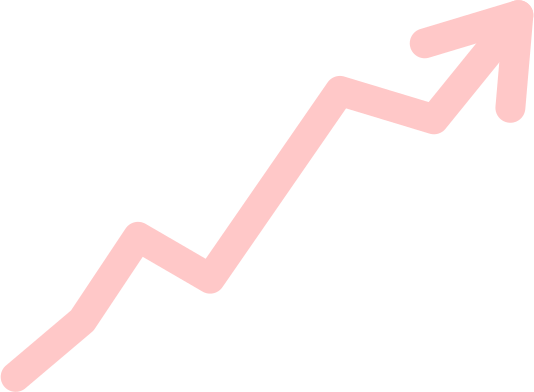
\includegraphics[height=0.2\textheight]{./images/general/growing}%

\end{frame}

%%%%%%%%%%%%%%%%%%%%%%%%%%%%%%%%%%%%%%%%%%%%%%%%%%%%%%%%%%%%%%%%%%%%%
\begin{frame}{Open in science}

% science
\quoteText{Software [...] developed as part of novel methods is as 
    important for the method's implementation [...]
    Such software [...] must be made available to readers upon publication.}
  {Social software, Nature Methods 4, 189, 2007}%
  {http://www.nature.com/nmeth/journal/v4/n3/full/nmeth0307-189.html}
% Software that is custom-developed as part of novel methods is as important
% for the method's implementation as reagents and protocols.
% Such software, or the underlying algorithms, must be made available to readers upon publication.

% continuation article: http://www.nature.com/nmeth/journal/v11/n3/full/nmeth.2880.html
% The usefulness of computational methods can be improved by releasing code and designing software
% that supports reproducible research.
% An open implementation that supports reproducible research not only provides confidence
% in the performance of a method but increases the likelihood
% that other researchers can use and build upon it.

% derived artile: http://opensource.com/life/14/6/respected-journal-makes-transition-open-science

% edu
\quoteText{The opposite of ‘open’ isn’t closed. The opposite of open is ‘broken.’}%
  {Cable Green (quoting John Wilbanks) at Open Scotland Summit 2013}
  {https://openscot.wordpress.com/2013/10/09/open-scotland-report-and-actions/}
% John Wilbanks and cited by Cable Green, The Obviousness of Open Policy:
% https://ronmader.wordpress.com/2012/09/06/open/
% Cable Green, at Open Scotland Summit, Open Scotland Report and Actions, July 4, 2013:
% https://openscot.wordpress.com/2013/10/09/open-scotland-report-and-actions/

\bigskip
\bigskip

\centering
\includegraphics[height=0.4\textheight]{./images/general/open_science}%
\\
\tiny
Image credit: \href{https://opensource.com/}{Opensource.com}


\end{frame}


\newcommand{\coursesTitle}{North Carolina State University}


%%%%%%%%%%%%%%%%%%%%%%%%%%%%%%%%%%%%%%%%%%%%%%%%%%%%%%%%%%%%%%%%%%%%%
\begin{frame}{Teaching enterprise software}

\begin{block}{Requirements}
\begin{itemize}
 \item Students needs to know enterprise software
 \item Minimize what students need to learn
\end{itemize}
\end{block}

\begin{block}{Result}
\begin{itemize}
 \item Students are taught single proprietary software
\end{itemize}
\end{block}

\centering
\Large
enterprise = proprietary?

\end{frame}


%%%%%%%%%%%%%%%%%%%%%%%%%%%%%%%%%%%%%%%%%%%%%%%%%%%%%%%%%%%%%%%%%%%%%
\begin{frame}{\coursesTitle: Course descriptions}


% \url{https://cnr.ncsu.edu/geospatial/academics/courses/}

% old
% https://web.archive.org/web/20160108192830/https://cnr.ncsu.edu/geospatial/education/courses/
% 12 std curses
% 1 mentions open and 1 mentions specific open but at the same time both particular proprietary
% 7 proprietary from a single vendor
% two other sw from diff vendor are mentioned MS SQL Server and Oracle
% 1 mentions Python (coupled with proprietary)
% -> more than half (7/12) of the courses explicitly mentions software from a single vendor
% -> one third (3/12) mentions different software, from that one is Python and two other Oracle and MS SQL Server
% -> the same three mention some open source software, from that one is Python, one is GRASS GIS, and one is general mention of open source software
% -> the same three at the same time make use of proprietary software
% -> 12 courses, 7 mention software, 7 mention proprietary sw, 3 some open source, 1 field specific (relevant) software, 0 open without using proprietary

% new
% https://web.archive.org/web/20171011010652/https://cnr.ncsu.edu/geospatial/academics/courses/
% 12 course
% 2 software, 1 proprietary, 1 some open (Python), 0 field specific (relevant) software, 0* open without using proprietary

\pgfplotstableread[row sep=\\,col sep=&]{
    val & old & new \\
    courses     & 12 & 12 \\
    mentions software     & 7 & 2 \\
    proprietary    & 7 & 1 \\
    some open & 3 & 1 \\
    field specific open  & 1 & 0  \\
    open only  & 0 & 0 \\
    }\mydata

% red - blue
% \definecolor{old}{HTML}{C0504D}
% \definecolor{new}{HTML}{4F81BD}

% viridis
% \definecolor{old}{HTML}{404186}
% \definecolor{new}{HTML}{6ACD5A}

% plasma
% \definecolor{old}{HTML}{16068A}
% \definecolor{new}{HTML}{FCA834}

% magma
% \definecolor{old}{HTML}{360F6B}
% \definecolor{new}{HTML}{F56C5B}

\definecolor{old}{HTML}{595959}
\definecolor{new}{HTML}{7CCD7C}

Mentions of software in the course description.*

\begin{tikzpicture}
    \begin{axis}[
            xbar,
            symbolic y coords={open only, field specific open,some open, proprietary,mentions software,courses},
            ytick=data,
            nodes near coords,
            legend pos=south east,
            reverse legend,
        ]
        \addplot+[fill=new,color=new] table[y=val,x=new]{\mydata};
        \addlegendentry{2017}
        \addplot+[fill=old,color=old] table[y=val,x=old]{\mydata};
        \addlegendentry{2016}

    \end{axis}
\end{tikzpicture}

*There are just short descriptions, not the actual course content.

\end{frame}


%%%%%%%%%%%%%%%%%%%%%%%%%%%%%%%%%%%%%%%%%%%%%%%%%%%%%%%%%%%%%%%%%%%%%
\begin{frame}{Including open}

\begin{block}{Maybe open is special}
\begin{itemize}
 \item Does teaching Python as scripting language of a proprietary
       software count as teaching open source?
       \begin{itemize}
       \item Most programming languages are open source.
       \end{itemize}
 \item Does teaching Open Geospatial Consortium (OGC) standards
       count as including open?
       \begin{itemize}
       \item Everybody should use standards.
       \end{itemize}
\end{itemize}
\end{block}

\Large
\textrightarrow Explicitly including open into class curriculum.

\end{frame}


%%%%%%%%%%%%%%%%%%%%%%%%%%%%%%%%%%%%%%%%%%%%%%%%%%%%%%%%%%%%%%%%%%%%%
\begin{frame}{Explicitly mentioning open}

\begin{block}{Maybe open is special}
\begin{itemize}
 \item Different business and support models
 \item Different development goals
 \item Role of community
 \item ...
\end{itemize}
\end{block}

\end{frame}

%%%%%%%%%%%%%%%%%%%%%%%%%%%%%%%%%%%%%%%%%%%%%%%%%%%%%%%%%%%%%%%%%%%%%
\begin{frame}{Explicitly mentioning open: Web}

\begin{block}{University of Kentucky: New Maps Plus graduate program}
\begin{itemize}
 \item Explicitly mentions open source source software
 \item Some OpenStreetMap
 \item Mostly focused on web
\end{itemize}
\end{block}

But open versus proprietary is not web versus desktop.

\textrightarrow To cover open, more than web is needed.

\textrightarrow
(Pure) OpenStreetMap is not replacement
for proprietary analytical GIS.

\end{frame}

%%%%%%%%%%%%%%%%%%%%%%%%%%%%%%%%%%%%%%%%%%%%%%%%%%%%%%%%%%%%%%%%%%%%%
\begin{frame}{OpenStreetMap as part of analysis}

\begin{block}{}
\emph{Towards an Automated Comparison of OpenStreetMap
with Authoritative Road Datasets.}
MA Brovelli, M Minghini, ME Molinari, P Mooney
Transactions in GIS 21 (2), 191-206
\begin{itemize}
 \item research by Brovelli et al.
 \item completeness and spatial accuracy of OpenStreetMap
 \item using GRASS GIS for analysis
\end{itemize}
\end{block}

\end{frame}

%%%%%%%%%%%%%%%%%%%%%%%%%%%%%%%%%%%%%%%%%%%%%%%%%%%%%%%%%%%%%%%%%%%%%
\begin{frame}{\coursesTitle: New PhD courses}


\begin{block}{\href{https://cnr.ncsu.edu/geospatial/academics/phd-in-geospatial-analytics/}%
  {Ph.D. in Geospatial Analytics}}
\begin{itemize}
 \item GIS 711: Geospatial Data Management:
...Applied experience in the architecture of geospatial data management \textbf{including open source options}...

\item GIS 715: Geovisualization:
...This course provides a systematic framework of visualization design principles based on the human visual system and \textbf{explores open-source geospatial data visualization tools}...
\end{itemize}

\end{block}

But open is not part of the vision.

\textrightarrow We need to decide and specify why we are including open.

\end{frame}

\newcommand{\geoforalllab}{NCSU GeoForAll Lab}

%%%%%%%%%%%%%%%%%%%%%%%%%%%%%%%%%%%%%%%%%%%%%%%%%%%%%%%%%%%%%%%%%%%%%
\begin{frame}{\geoforalllab: The idea}

\begin{columns}[c]

\column{.45\textwidth}

\begin{itemize}
 \item lectures:
 \begin{itemize}
  \item theory, concepts
  \item software-independent
 \end{itemize}
 \item labs and assignments:
 \begin{itemize}
  \item relate to given lecture
  \item hands-on, practical
  \item students use software
%   \item software-dependent
 \end{itemize}
\end{itemize}

\column{.45\textwidth}

\bigskip

\centering

\includegraphics[width=0.5\textwidth]{./images/general/bulp}%
\\
\tiny
\color{gray}
Image credit: \href{https://openclipart.org}{Openclipart}

\end{columns}

\end{frame}

%%%%%%%%%%%%%%%%%%%%%%%%%%%%%%%%%%%%%%%%%%%%%%%%%%%%%%%%%%%%%%%%%%%%%
\begin{frame}{The problem}

% Students use software in labs and for assignments.

% In labs and for assignments are software-dependent.

\begin{itemize}
 \item students are becoming (only) software users instead of scientists
 \item students mix software details and general concepts
 \begin{itemize}
  \item saying Shapefile or feature class instead of
    \href{http://www.opengeospatial.org/ogc/glossary/v}{\emph{vector}} data%
    % http://www.opengeospatial.org/ogc/glossary/v
    % http://www.opengeospatial.org/ogc/glossary/f
    % http://www.opengeospatial.org/ogc/glossary/s
    % http://www.opengeospatial.org/ogc/glossary/r
    \ldots
\end{itemize}
 \item bonding with software limits flexibility
 \item software promotes software/vendor-specific formats/technologies
 \item single software choice limits explored algorithms

\end{itemize}

\end{frame}


%%%%%%%%%%%%%%%%%%%%%%%%%%%%%%%%%%%%%%%%%%%%%%%%%%%%%%%%%%%%%%%%%%%%%
\begin{frame}{The solution}

\begin{itemize}
 \item lectures:
 \begin{itemize}
  \item theory, concepts
  \item software-independent
 \end{itemize}
 \item labs and assignments:
 \begin{itemize}
  \item relate to given lecture
  \item hands-on, practical
  \item \alert<1>{students use two different software packages}
  \pause
  \item similar task in both
  \end{itemize}
\pause
\item opportunity to see what is a general concept
        and what is specific to a~particular software
\item they gain flexibility to choose optimal solutions for their future work
\item more time needed, but worth it
\end{itemize}

\end{frame}



%%%%%%%%%%%%%%%%%%%%%%%%%%%%%%%%%%%%%%%%%%%%%%%%%%%%%%%%%%%%%%%%%%%%%
\begin{frame}{\geoforalllab: Courses}

\begin{columns}[c]

\column{.55\textwidth}

\begin{block}{\href{http://courses.ncsu.edu/gis582/common/}%
  {Geospatial Analysis and Modeling}}
\begin{itemize}
 \item started in 2008
 \item on-campus and distance education
 \item every semester 30-60 students
 \item software:
 \begin{itemize}
   \item \href{http://grass.osgeo.org}{GRASS GIS}
   \item ArcGIS
 \end{itemize}
\end{itemize}
\end{block}

\column{.40\textwidth}

\includegraphics[width=\textwidth]{./images/edu/secref}%

\end{columns}

\end{frame}

%%%%%%%%%%%%%%%%%%%%%%%%%%%%%%%%%%%%%%%%%%%%%%%%%%%%%%%%%%%%%%%%%%%%
\begin{frame}{\geoforalllab: Courses}

\begin{columns}[c]

\column{.65\textwidth}

\begin{block}{\href{http://courses.ncsu.edu/mea592/common/}%
  {Multidimensional Geospatial Modeling}}

\begin{itemize}
 \item software:
 \begin{itemize}
   \item \href{http://grass.osgeo.org}{GRASS GIS}
   {\scriptsize
    often with new features such as
    \href{http://grass.osgeo.org/grass70/manuals/temporalintro.html}{Temporal Framework}
    (\href{http://grass.osgeo.org/grass7/}{GRASS GIS 7})
   }
  \item + whatever the students need, e.g.~%
    \href{http://www.liblas.org/}{libLAS}
 \end{itemize}

 \item new technologies:
   \href{http://geospatial.ncsu.edu/osgeorel/tangible-landscape.html}%
   {Tangible Landscape}

\end{itemize}

\end{block}

\column{.3\textwidth}

\href{https://www.youtube.com/channel/UCc37pVh-WE46Xkqeq-KZQsA}{%
\includegraphics[height=0.65\textheight]{./images/edu/tangible}%
}

\end{columns}

\href{https://www.lib.ncsu.edu/stories/large-scale-visualization-geospatial-data}{%
\includegraphics[width=\textwidth]{./images/edu/hunt_vis}%
}

\end{frame}

%%%%%%%%%%%%%%%%%%%%%%%%%%%%%%%%%%%%%%%%%%%%%%%%%%%%%%%%%%%%%%%%%%%%%
\begin{frame}{Related workshop: Tangible Landscape}

\centering
\includegraphics[height=0.6\textheight]{./images/tangible/sod_workshop}

\Large

by Anna Petrasova
Byron North,
Sun, 9:00am

\end{frame}


%%%%%%%%%%%%%%%%%%%%%%%%%%%%%%%%%%%%%%%%%%%%%%%%%%%%%%%%%%%%%%%%%%%%%
\begin{frame}{\geoforalllab: Courses}


\begin{block}{\href{http://ncsu-osgeorel.github.io/uav-lidar-analytics-course/}%
  {UAV/lidar Data Analytics}}
\begin{itemize}
 \item under development
 \item Agisoft PhotoScan in class (proprietary), \href{http://opendronemap.org/}{OpenDroneMap} in projects (open source)
\end{itemize}

Related talk:
OpenDroneMap by Dakota Benjamin (Byron North, Sat, 3:35pm)

\end{block}

\begin{columns}[c]

\column{.45\textwidth}
\includegraphics[height=0.5\textheight]{./images/edu/dem}
\column{.45\textwidth}
\hspace{0.2\textwidth}
\rotatebox{-90}{\includegraphics[width=0.5\textheight]{./images/edu/uav}}
\end{columns}

\end{frame}


%%%%%%%%%%%%%%%%%%%%%%%%%%%%%%%%%%%%%%%%%%%%%%%%%%%%%%%%%%%%%%%%%%%%%
\begin{frame}{\geoforalllab: Courses}

\begin{block}{Tools for open science course}

\begin{itemize}
 \item Course dedicated to
 \begin{itemize}
  \item exploring important role FOSS plays in science
  \item overview of tools and methods common in FOSS and desperately needed in science
  \item open source, open access, open data, open standards, open...
  \item reusability and reproducibility are standard in FOSS
 \end{itemize}
\end{itemize}

\end{block}

\smallskip

\centering
\includegraphics[height=0.4\textheight]{./images/general/open_up_book}%
\\
\tiny
Image credit: \href{https://opensource.com/}{Opensource.com}

\end{frame}



%%%%%%%%%%%%%%%%%%%%%%%%%%%%%%%%%%%%%%%%%%%%%%%%%%%%%%%%%%%%%%%%%%%%%
\begin{frame}{\geoforalllab: Teaching materials}

\begin{itemize}
 \item license: \href{https://creativecommons.org/licenses/by-sa/4.0/}{CC BY-SA}
 \item Git (GitHub hosted)
  {\scriptsize for revision control, collaboration and sharing source code}
 \item registered in \href{http://www.osgeo.org/educational_content}{OSGeo Educational Content Inventory}
 {\small Now being transfered to a new website}
\end{itemize}

\href{http://geospatial.ncsu.edu/osgeorel/courses.html}%
  {
  \begin{minipage}[b]{0.2\textwidth}
    \begin{center}
      \includegraphics[height=0.9\textwidth]{./images/edu/osgeorel_courses_qr}\\
      \tiny \tt geospatial.ncsu.edu/\\osgeorel/courses.html
    \end{center}
  \end{minipage}
  }
\hfill%
\href{http://courses.ncsu.edu/gis582/common/grass/data_models.html}{%
\includegraphics[height=0.2\textwidth]{./images/edu/osgeorel_courses_header}
\hfill
\includegraphics[height=0.2\textwidth]{./images/edu/osgeorel_courses_example}%
}

\end{frame}

%%%%%%%%%%%%%%%%%%%%%%%%%%%%%%%%%%%%%%%%%%%%%%%%%%%%%%%%%%%%%%%%%%%%%
\begin{frame}{Paper}

\href{http://www.mdpi.com/2220-9964/4/2/942}%
  {\emph{Integrating Free and Open Source Solutions into Geospatial Science Education}
  \hfill \footnotesize \color{gray} Open Access}

Vaclav Petras\n{1,\,4},
Anna Petrasova\n{1,\,4},
Brendan Harmon\n{2,\,4},
\mbox{Ross K. Meentemeyer}\n{3,\,4},
and Helena Mitasova\n{1,\,4}

\medskip

In: \href{http://www.mdpi.com/journal/ijgi/special_issues/science-applications}%
{\emph{ISPRS International Journal of Geo-Information}}. 2015.
% Special Issue "Open Geospatial Science and Applications"

\bigskip

\href{http://dx.doi.org/10.3390/ijgi4020942}%
  {
  \begin{minipage}[b]{0.2\textwidth}
    \begin{center}
      \includegraphics[height=0.9\textwidth]{./images/edu/paper_qr}\\
      \tiny \tt doi:10.3390/ijgi4020942
    \end{center}
  \end{minipage}
  }
\hfill
\includegraphics[height=0.2\textwidth]{./images/edu/paper_picture}

\end{frame}


%%%%%%%%%%%%%%%%%%%%%%%%%%%%%%%%%%%%%%%%%%%%%%%%%%%%%%%%%%%%%%%%%%%%%
\begin{frame}{\geoforalllab: Data -- OpenStreetMap}

\begin{flushright}
Context: Advanced master and PhD courses
\end{flushright}

\begin{itemize}
 \item Students often come with knowledge of OpenStreetMap.
 \item Often they think it is a name of an ESRI basemap.
\end{itemize}

Too late to have introduction to geography
with OpenStreetMap.

Seeking ideas for introducing OpenStreetMap into graduate level courses
(now: part of student projects).

\end{frame}

%%%%%%%%%%%%%%%%%%%%%%%%%%%%%%%%%%%%%%%%%%%%%%%%%%%%%%%%%%%%%%%%%%%%%
\begin{frame}[fragile]{Standardized Sample Datasets for Teaching}

\begin{itemize}
 \item region specific datasets limit sharing of hands-on teaching material
 \item new version of North Carolina
 \begin{itemize}
  \item commonly available data, frequently used in examples
  \item standardized names such as \textit{elevation}, \textit{streets}, or \textit{lakes}
  \begin{itemize}
   \item rather than \textit{srtm}, \textit{dem\_10m}, \textit{streets\_como}
  \end{itemize}
 \end{itemize}
 \item \alert{different datasets should use the same standardized names}
 \item challenges:
 \begin{itemize}
  \item attributes, coordinates, values, extents, resolutions, (natural) languages
 \end{itemize}

\end{itemize}

\smallskip

\begin{columns}[c]

 \column{.45\textwidth}
\scriptsize
\begin{verbatim}
g.region raster=elevation
r.relief input=elevation output=shade
\end{verbatim}
\begin{verbatim}
d.shade shade=shade color=elevation
\end{verbatim}
\vfill\hfill\hfill
\href{http://grasswiki.osgeo.org/wiki/GRASS_GIS_Standardized_Sample_Datasets}{%
$\blacktriangleright$ grasswiki.osgeo.org}

\column{.40\textwidth}
 \includegraphics[width=\textwidth]{./images/dataset/std_dataset_piemonte_shaded_elevation}%
\end{columns}


\end{frame}



%%%%%%%%%%%%%%%%%%%%%%%%%%%%%%%%%%%%%%%%%%%%%%%%%%%%%%%%%%%%%%%%%%%%%
\begin{frame}{Standardized Sample Dataset: North Carolina, USA}

\begin{center}
\includegraphics[width=\textwidth]{./images/dataset/std_dataset_nc_stripe.png}
\end{center}


Helena Mitasova\n{1} and Markus Neteler\n{2}, authors of
\mbox{\href{http://grassbook.org/}{\it Open Source GIS: A GRASS GIS Approach}}
{\scriptsize (fourth edition in preparation)}

\bigskip

{\scriptsize
$^1$\href{http://www.meas.ncsu.edu/}%
{Department of Marine, Earth, and Atmospheric Sciences,
North Carolina State University, USA}

$^2$\href{http://gis.cri.fmach.it/}%
% GIS and Remote Sensing Unit
{Research and Innovation Centre, Fondazione Edmund Mach, Italy}
}

\end{frame}

%%%%%%%%%%%%%%%%%%%%%%%%%%%%%%%%%%%%%%%%%%%%%%%%%%%%%%%%%%%%%%%%%%%%%
\begin{frame}{Standardized Sample Dataset: Czech Republic}

\begin{center}
\includegraphics[width=\textwidth]{./images/dataset/std_dataset_cz_stripe.png}
\end{center}

\href{http://gismentors.eu/}{Martin Landa\n{*} and Jachym Cepicky from GISMentors}

\bigskip

$^*$\href{http://geomatics.fsv.cvut.cz/research/osgeorel/}%
{\scriptsize
OSGeoREL
at Czech Technical University in Prague,
Faculty of Civil Engineering
}

\end{frame}

%%%%%%%%%%%%%%%%%%%%%%%%%%%%%%%%%%%%%%%%%%%%%%%%%%%%%%%%%%%%%%%%%%%%%
\begin{frame}{Standardized Sample Dataset: Piedmont, Italy}
% English: Piedmont [ˈpiːdmɒnt] PEED-mont
% Italian: Piemonte [pjeˈmonte]

\begin{center}
\includegraphics[width=\textwidth]{./images/dataset/std_dataset_it_stripe.png}
\end{center}


Luca Delucchi and Markus Neteler

{\scriptsize
\href{http://gis.cri.fmach.it/}{Research and Innovation Centre, Fondazione Edmund Mach, Italy}
}

\end{frame}

%%%%%%%%%%%%%%%%%%%%%%%%%%%%%%%%%%%%%%%%%%%%%%%%%%%%%%%%%%%%%%%%%%%%%
\begin{frame}{Standardized Sample Dataset: Puerto Rico}

\begin{center}
\includegraphics[width=\textwidth]{./images/dataset/std_dataset_pr_stripe.png}
\end{center}

Keren Cepero-Perez

{\scriptsize
\href{http://www.meas.ncsu.edu/}%
{Department of Marine, Earth, and Atmospheric Sciences,
North Carolina State University, USA}
}

\end{frame}



%%%%%%%%%%%%%%%%%%%%%%%%%%%%%%%%%%%%%%%%%%%%%%%%%%%%%%%%%%%%%%%%%%%%%
\begin{frame}{Standardized Sample Dataset: Data sources}

\begin{itemize}
 \item buildings, roads, ...: OpenStreetMap
 \item orthophoto: OpenAerialMap?
 \item digital elevation model: OpenTopography?
\end{itemize}

\end{frame}


%%%%%%%%%%%%%%%%%%%%%%%%%%%%%%%%%%%%%%%%%%%%%%%%%%%%%%%%%%%%%%%%%%%%%
\begin{frame}{}

\begin{block}{Summary}
 \begin{itemize}
  \item teaching 2 software packages to improve students' geospatial skills
  \item OpenStreetMap as dataset and way of doing things
  \item GeoForAll (\texttt{geoforall.org})
 \end{itemize}

\end{block}

\bigskip

\begin{columns}[c]

\column{.45\textwidth}

\begin{block}{Contact}
\begin{tabular}{rl}
 Homepage: &\href{https://wenzeslaus.github.io}{\texttt{wenzeslaus.github.io}}
 \\
 GitHub: &\texttt{wenzeslaus}
 \\
 Twitter: &\texttt{@vaclavpetras}
\end{tabular}
\end{block}

\column{.45\textwidth}

\centering
\includegraphics[width=0.5\textwidth]{./images/general/slides_qr}

\end{columns}

\small
Acknowledgement:
Scholarship for State of the Map US 2017

\end{frame}

\end{document}
